\chapter{Code Smell Refactoring}

\paragraph{Code Smell: Long Method}


Die Klasse \textit{WordGenerator} ist dafür zuständig alle möglichen Wörter in einem Raster von Buchstaben zu finden. Dafür hat sie zwei Funktionen welche jeweils ca. 50 Zeilen lang sind. Beide Funktionen sind durch viele Schleifen sehr unübersichtlich und fallen unter die Long Method Code Smells. Zum Refactoren des Code Smells wird die Funktion zuerst mittels Extract Method in kleinere Funktionen unterteilt. Dabei wurde direkt noch die If-Abfrage zur besseren Lesbarkeit umgedreht. Die extrahierten Methoden sind in Abb.~\ref{Abb:ExtractMethod} in Grün und Orange markiert. (Commit:~\href{https://github.com/EinToni/Wortfinder/commit/b6e3b31e4ef7b597863bc2be073f9e136d4b9594}{b6e3b31e4ef7b597863bc2be073f9e136d4b9594})

\begin{figure}[!ht]
  \centering
  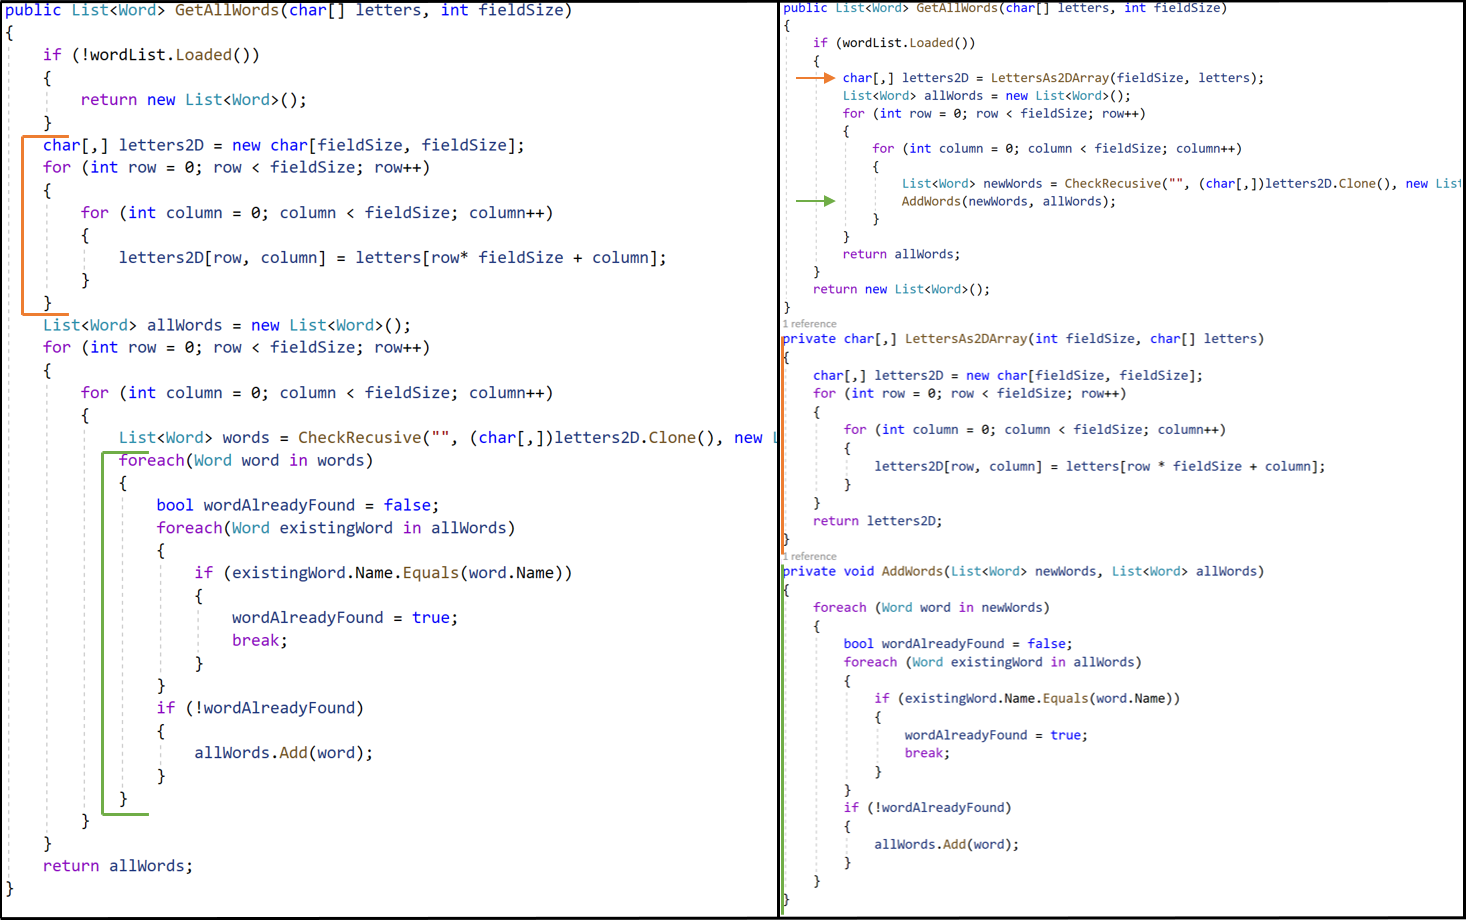
\includegraphics[width=\textwidth]{Bilder/ExtractMethod.PNG}
  \caption[Anwendung des Extract Method Refactoring]{Anwendung des Extract Method Refactoring (\href{https://github.com/EinToni/WortfinderDoku/blob/main/Bilder/ExtractMethod.png}{Link})}
  \label{Abb:ExtractMethod}
\end{figure}

Danach fallen die zwei gleichen Schachtelungen der for-Schleifen auf. Dabei wird in der Funktion \textit{LettersAs2DArray} das Eingabe-Array zu einem 2D-Array umstrukturiert. Da die Buchstaben in einen Raster angeordnet sind, ist so ein Iterieren und suchen von Nachbarn einfacher vorstellbar. Da zwischenzeitlich allerdings die \textit{Coordinate} Klasse eingefügt wurde, welche das Prüfen auf Nachbarschaft zweier Koordinaten übernimmt, lässt sich dieser Code vereinfachen. Das durchlaufen des 2D Arrays (Abb.~\ref{Abb:CodeVereinfachen} Orange markiert) wird somit durch ein einmaliges durchlaufen des Ursprünglichen Arrays ersetzt. Die \textit{LettersAs2DArray} Funktion wird hier nur noch für den Aufruf an die nächste Funktion benötigt und kann nach dessen Refactorings komplett entfernt werden. Außerdem kann die in Grün markierte Funktionalität, welche überprüft ob ein Wort schon in der Liste ist, ebenfalls durch Extract-Method ausgelagert werden. Es ergibt sich somit folgender Code (Commit:~\href{https://github.com/EinToni/Wortfinder/commit/f733dabc6753529e597408cc8c76ea0a39a1ff8e}{f733dabc6753529e597408cc8c76ea0a39a1ff8e}):

\begin{figure}[!ht]
  \centering
  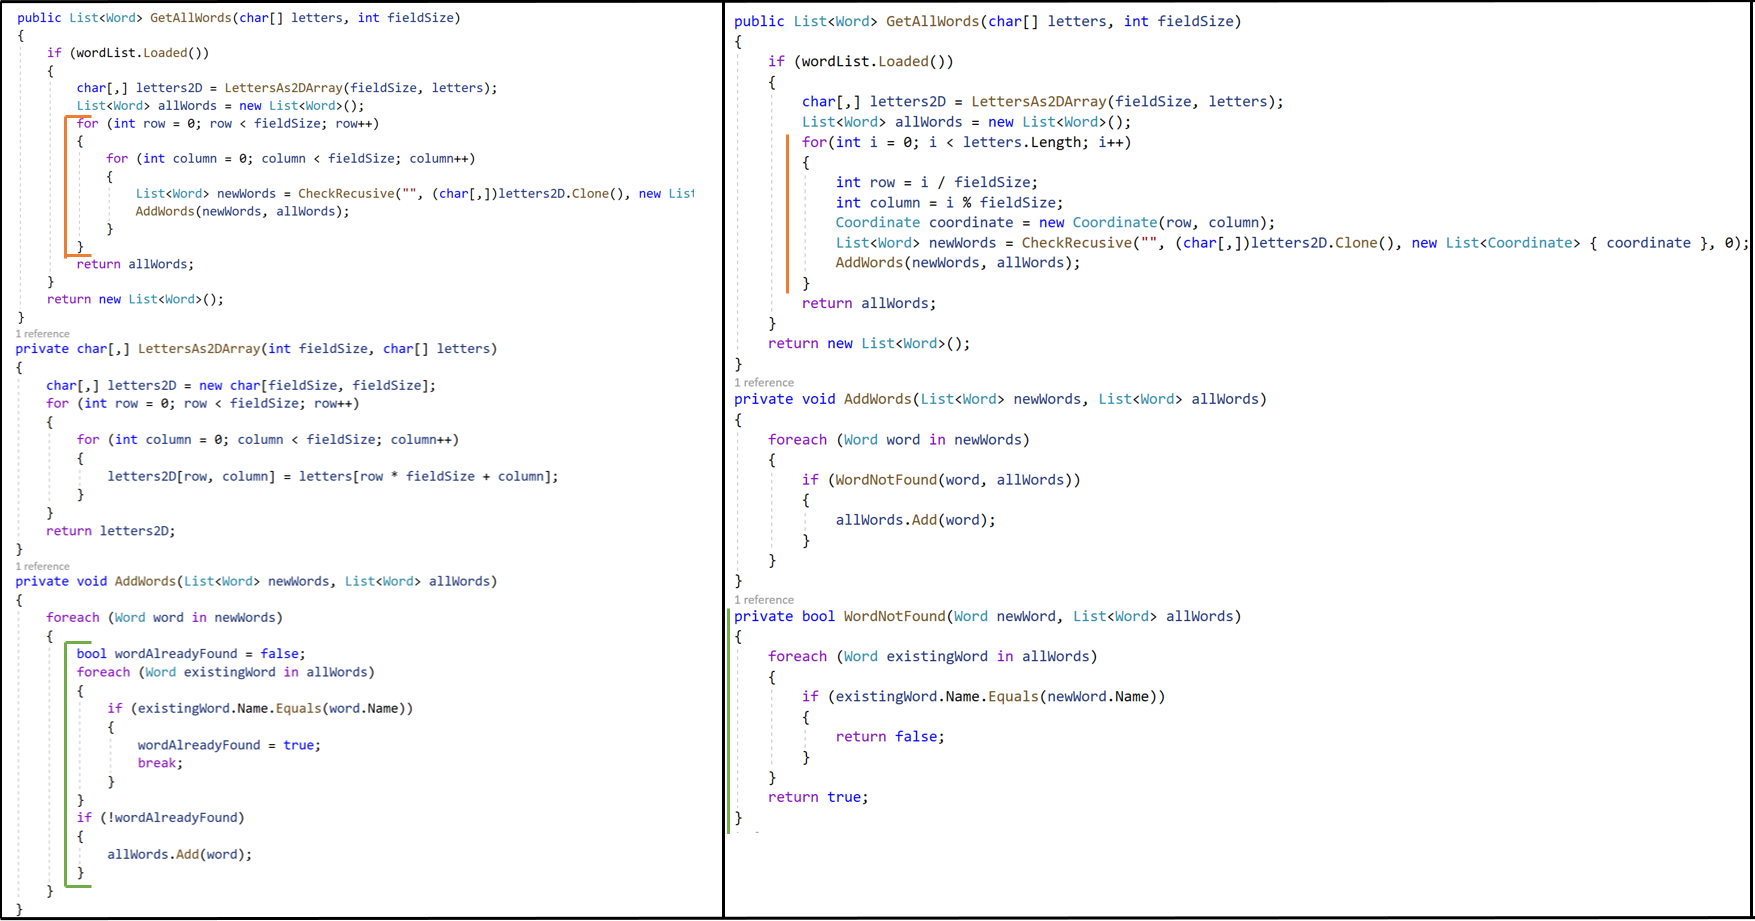
\includegraphics[width=\textwidth]{Bilder/CodeVereinfachen.PNG}
  \caption[Extract Method und Code Vereinfachung]{Extract Method und Code Vereinfachung (\href{https://github.com/EinToni/WortfinderDoku/blob/main/Bilder/CodeVereinfachen.png}{Link})}
  \label{Abb:CodeVereinfachen}
\end{figure}

In der zweiten Funktion wird ebenfalls mit Extract Method begonnen (Abb.~\ref{Abb:ExtractMethod2}). Dabei werden zwei verschachtelte Schleifen ausgelagert, in welchen die betroffene Methode Rekursiv wieder aufgerufen wird. Da bei der Rekursion alle Parameter mitgegeben werden müssen, ist ein komplettes auslagern unvorteilhaft, da in diese neue Methode dann ebenfalls alle Parameter weitergegeben werden müssten. Daher wird nur der Teil in eine neue Methode verschoben, welcher alle benachbarten Positionen im Buchstabengitter findet (Orange markiert), Commit: \href{https://github.com/EinToni/Wortfinder/commit/23cf0b7d1165c1d17235d68f8fca35682ba233ad}{23cf0b7d1165c1d17235d68f8fca35682ba233ad}):
\newpage
\begin{figure}[!ht]
  \centering
  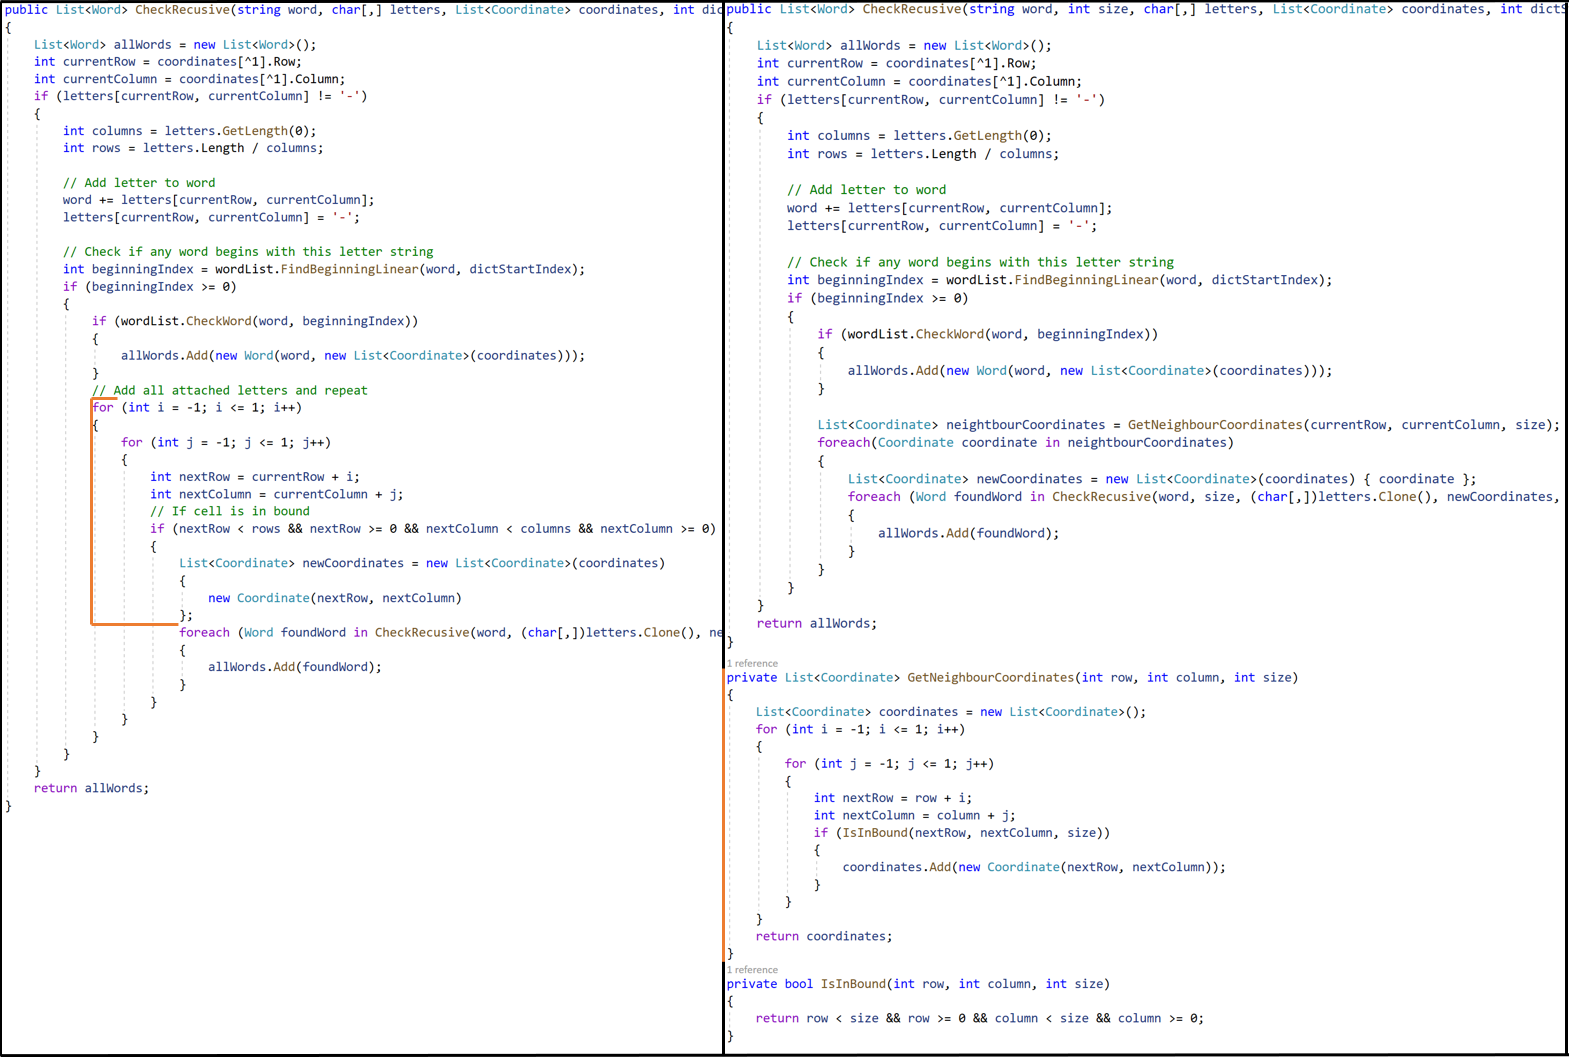
\includegraphics[width=\textwidth]{Bilder/ExtractMethod2.PNG}
  \caption[Extract Method]{Extract Method (\href{https://github.com/EinToni/WortfinderDoku/blob/main/Bilder/ExtractMethod2.png}{Link})}
  \label{Abb:ExtractMethod2}
\end{figure}

Danach wird auch hier das zweidimensionale Array durch ein eindimensionales ersetzt. Außerdem lässt sich das innerste \textit{foreach} durch die Nutzung von der \textit{AddWords} Funktion ersetzen, welche durch Extract-Method in der ersten Funktion entstanden ist. 


Die Gesamtlänge des Codes hat sich durch Anwenden der Refactorings nicht verkürzt. Dafür wurde die Lesbarkeit sowie die Wiederverwendbarkeit wesentlich gesteigert. Die fertigen Funktionen sind in Commit \href{https://github.com/EinToni/Wortfinder/commit/e56ec221727039af2f0b6c06985f3b0edf8bdf3c}{e56ec221727039af2f0b6c06985f3b0edf8bdf3c} einsehbar.

\newpage
\paragraph{Code Smell: Duplicated Code}

Es werden sowohl vorgeladene Spiele, wie auch Highscores auf der Festplatte lokal gespeichert und beides soll nicht editierbar sein. Daher lädt und speichert die Klasse \textit{ScoreDataController} die Highscores sowie \textit{GameDataController} die vorbereiteten Spiele. Beide beinhalten dabei den gleichen Code für die Ent-/Verschlüsselung. Dieser Duplicated Code wird mittels Extract-Method in eine neue Klasse ausgelagert welche die allgemeine Ent- und Verschlüsselung übernimmt. Da die neue Klasse nur Daten von einem Format in ein anderes Konvertiert, wird sie in der Clean Architecture bei den Aufrufenden Klassen in der Adapter-Schicht positioniert. (Commit: \href{https://github.com/EinToni/Wortfinder/commit/86e635fc6ddbd436ca012c21e3a00b9246248855}{86e635fc6ddbd436ca012c21e3a00b9246248855})

\paragraph{Weitere Refactorings}
Die Anwendung von weiteren Refactorings wird mittels folgender Abbildung, anhand der Methode \glqq FindBeginningLinear\grqq{} gezeigt. Die Methode wird mit einer Zahl und einem String aufgerufen und sucht in der Liste aller Wörter nach dem ersten Wort welches mit dem gegebenen String beginnt. Die Zahl gibt dabei den Start Index vor. Für eine möglichst schnelle Suche wurde die Methode am Anfang auf verschiedene Arten implementiert. Alle anderen Arten wurden aber verworfen und diese lineare Suche verwendet. Da es nun keine implementierten alternativen gibt, verwirrt der Namenszusatz \glqq Linear\grqq{} nur. Der Name wird daher mittels \glqq Rename Method\grqq{} verständlicher gemacht. 

Als zweites wird der Rückgabewert durch \glqq Replace Error Code with Exception\grqq{} angepasst. Somit wird, falls das Wort nicht in der Liste ist, keine $-1$ zurückgegeben, sondern eine Exception geworfen. Dadurch ist in der aufrufenden Methode keine Prüfung auf $\ge 0$ mehr notwendig, sondern wird mit einem try-catch-Block ersetzt.

Um die Lesbarkeit zu verbessern werden als letztes noch die Variablen \glqq begin\grqq{} und \glqq i\grqq{} zusammengefasst sowie umbenannt. Somit ist einfacherer Verständlich, dass es sich bei beidem um den Index in der Liste handelt und dass bei einem leeren String der Index Null sowie bei einem Fund der aktuelle Index zurückgegeben wird. 

(Commit: \href{https://github.com/EinToni/Wortfinder/commit/d194bb790cdc4e2638ff9ec223a89ecd0e51e515}{d194bb790cdc4e2638ff9ec223a89ecd0e51e515})

\begin{figure}[htb]
\centering
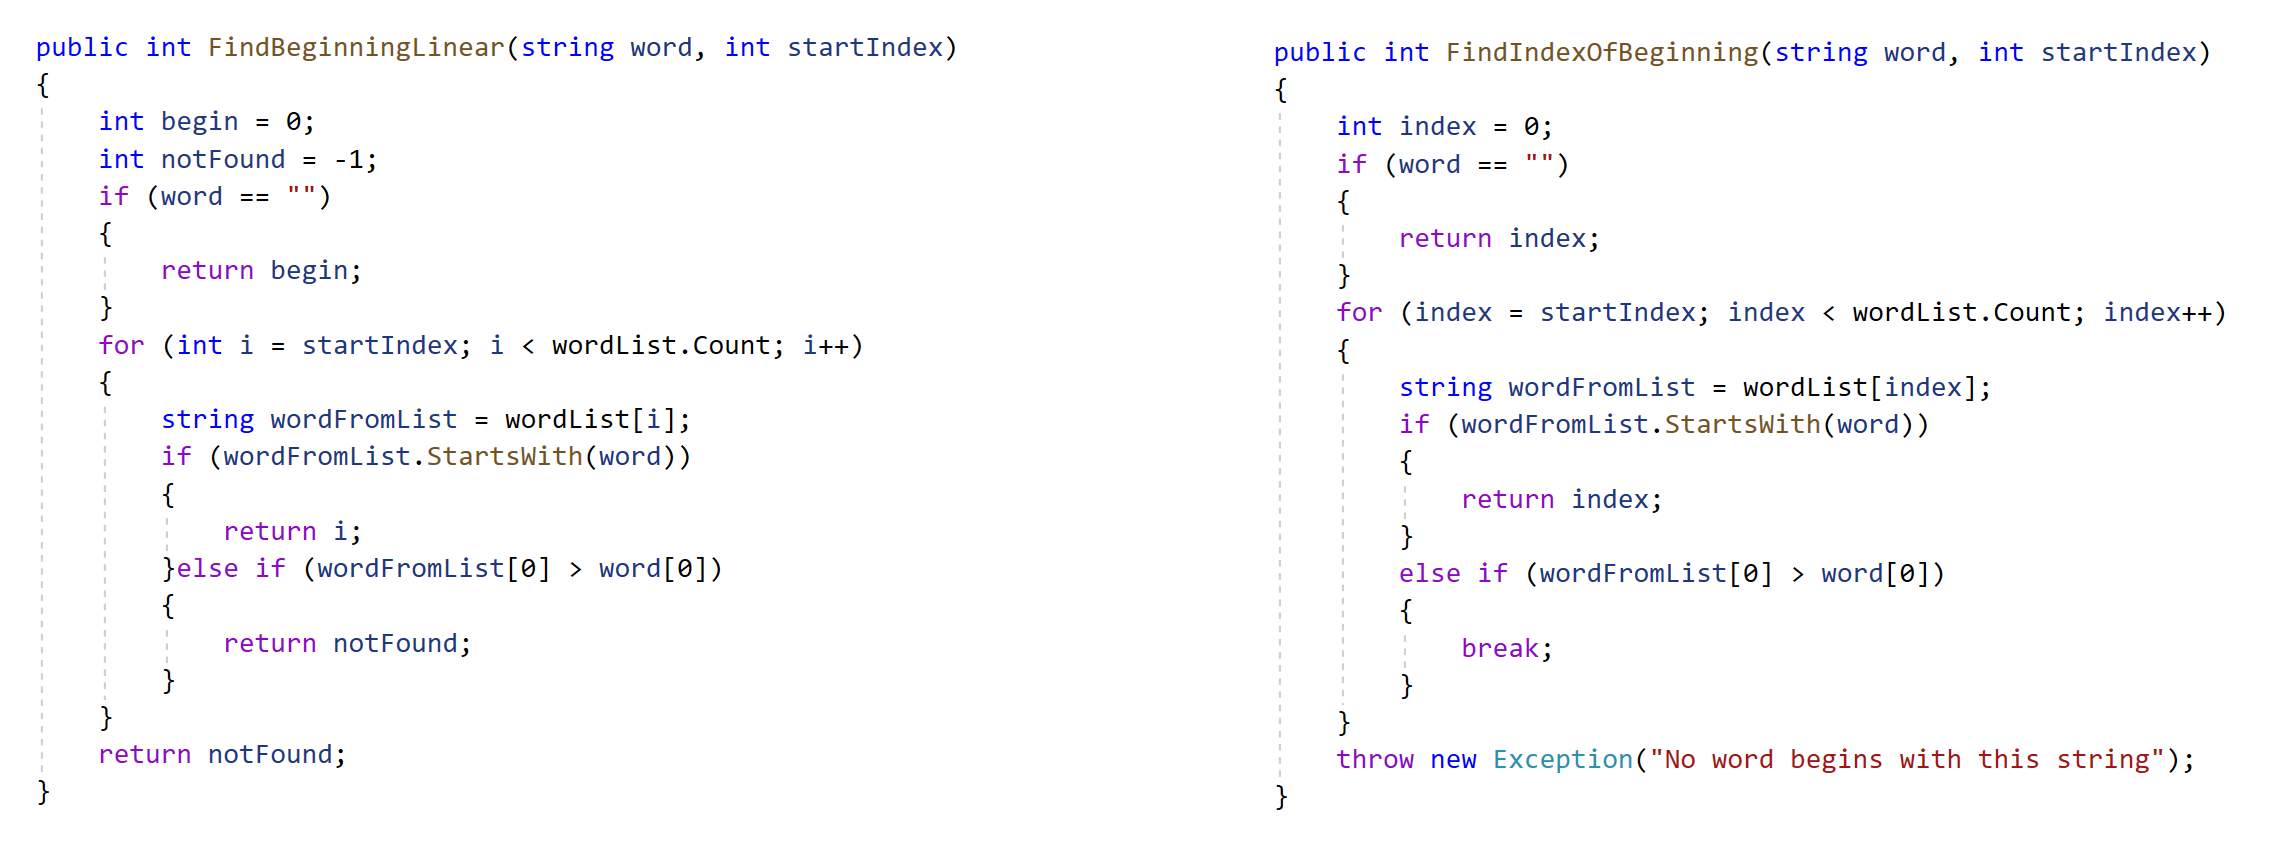
\includegraphics[width=\textwidth]{Bilder/Refactorings.PNG}
\caption{\label{Abb:Refactorings}Anwendung weiterer Refactoring}
\end{figure}



\endinput